\label{abstract}
%La miseriaccia ladra !!!
%- il problema affrontato;
%- il risultato conseguito;
%- la metodologia e/o tecnologia adottata;
%- il posizionamento o confronto rispetto ad eventuali risultati esistenti per lo stesso problema.

\paragraphh{Problema affrontato}
Il problema affrontato in questo lavoro di tesi è la realizzazione di implementazioni 
parallele ed efficienti per il triplo prodotto tra matrici sparse,
integrabili nella fase di setup dei solutori iterativi di sistemi lineari sparsi basati su metodi 
\emph{Algebraic Multi Grid} o \emph{AMG}.\\
L'esigenza di risolvere efficientemente sistemi lineari sparsi di grandi dimensioni 
insorge da applicazioni di calcolo scientifico come la risoluzione numerica di PDE su domini 2D o 3D, 
mediante griglie di discretizzazione, come descritto in \refbf{chIntro:PDE_intro}.\\
La sparsità dei sistemi lineari di tipo $Ax=b$ da risolvere è sfruttabile rappresentando 
della matrice $A$ in un formato sparso dove vengono omessi i valori nulli,
risparmiando memoria e limitando il processamento ai soli valori non zero,
dando un vantaggio notevole rispetto a tecniche algebriche convenzionali per matrici dense.\\
%TODO TODO accorcia o togli
La necessità di utilizzare solutori iterativi per questo tipo di sistemi in luogo di solutori diretti,
è dovuta alle proprietà di sparsità dei risultati intermedi, come verrà analizzato in \refbf{directVsIndirectSpLinSysSolvers}
e mostrato per alcuni casi in figura \refbf{fig:Efficient_Linear_System_Solvers_for_Mesh_Processing_densificationByDirectSolver}.\\
%insorge dal fatto che, a differenza della maggior parte dei solutori di tipo diretto, 
%viene preservata la proprietà di sparsità nelle matrici dei risultati intermedi,
%come visibile nella figura \refbf{fig:Efficient_Linear_System_Solvers_for_Mesh_Processing_densificationByDirectSolver},
%evitando di imbattersi in limitazioni di memoria e processamento per sistemi molto grandi e sparsi.\\
%
%I metodi \emph{AMG} godono di ottime caratteristiche di scalabilità 
%e possono essere applicati alla risoluzione di problemi discretizzati con griglie non strutturate,
%ad esempio mediante il metodo degli elementi finiti, come descritto in \refbf{multiGrid}.\\
%\voidLine
Al fine di ottimizzare l'esecuzione del prodotto di Galerkin (descritto dalla formula \refbf{eq:galerkin}) nella fase di setup 
dei metodi \emph{AMG} ho realizzato varie implementazioni per 
il triplo prodotto tra matrici sparse o {\bf{Sp}}arse{\bf{3}}{\bf{M}}atrixMatrix{\bf{M}}ultiplication (\emph{Sp3MM})
supportando la possibilità di inserire il lavoro in progetti fortran come \\\vvv{AMG4PSBLAS} (\refbf{amg4psblas}),
su cui è stato avviato un lavoro di integrazione.

\paragraphh{Tecniche utilizzate}
%formulazione principale usata
Il design delle implementazioni parallele per Sp3MM è stato guidato dalla formulazione \rowbyrow per il prodotto tra matrici sparse o\\
{\bf{Sp}}arse{\bf{M}}atrixMatrix{\bf{M}}ultiplication (\emph{SpMM}, descritta in \refbf{ChExistingTecqs:formulazioni}) introdotta da Gustavson \citebf{gustavson},
che consiste nel calcolare la $i$-esima riga del prodotto $A\cdot B = C$ come:	$c_{i*} = \sum\limits_{k \in I_i(A)}  a_{ik} \ast  b_{k*}$.\\
Al fine di realizzare efficientemente le moltiplicazioni scalari tra gli elementi di A e le righe di B: $a_{ik} \ast  b_{k*}$
è stato utilizzato un approccio basato su un accumulatore denso, descritto in \refbf{ssec:gustavsonDerivate}, 
dati gli ottimi risultati riscontrabili in una ricerca precedente \cite{intelSpMMDenseAccumulator}.\\
Il triplo prodotto è stato realizzato sia combinando una coppia di operazioni di SpMM, sia direttamente
estendendo la formulazione \rowbyrow con un approccio derivato dal lavoro di \citebf{Sp3MM4AMG}, come descritto in \refbf{chSpMMNum:directProduct}
\voidLine	
%formato matrici
Per la rappresentazione delle matrici sparse utilizzate è stato usato il formato\\{\bf{C}}ompressed{\bf{S}}parse{\bf{R}}ow,
dato che 
è considerabile un formato \emph{General-purpose} per matrici sparse, con un'occupazione in memoria proporzionale al numero di elementi non zero,
ed è correntemente impiegato \\in un'implementazione seriale di SpMM in \vvv{AMG4PSBLAS}.\\
%\voidLine
% What is OpenMP ?  OpenMP is a specification for a set of compiler directives, library routines, and environment variables that can be used to specify high-level parallelism in Fortran and C/C++ programs.
Tutte le implementazioni di Sp3MM sono state scritte in C
e per supportarne efficacemente una realizzazione parallela ho utilizzato le implementazioni offerte da GCC delle direttive OpenMP.\\
OpenMP comprende la specifica di un insieme di: 
direttive per compilatori, routines di libreria e variabili d'ambiente, utilizzabili per programmare ad alto livello regioni parallele in codici C/C++ e Fortran.
\voidLine
%symb kinds intro
Le realizzazioni parallele del prodotto tra matrici sparse necessitano di una fase iniziale, tipicamente denominata fase simbolica,
dove viene calcolata la dimensione del risultato finale (o un suo bound) per evitare di effettuare allocazioni dinamiche 
durante l'esecuzione parallela (di cui sono analizzate le problematiche a riguardo in \refbf{ChExistingTecqs:openMP_for_philosophy}).
La fase simbolica di SpMM può essere di tipo UpperBound, determinando un limite superiore al numero di elementi \nnz del risultato finale,
o di tipo accurato per una determinazione esatta.\\
%accurate symb
Per effettuare la fase simbolica accurata del prodotto tra matrici sparse (descritta nel capitolo \refbf{ChSymbProduct}),
sono state utilizzate strutture di ricerca efficienti come RedBlack (descritti in \refbf{chSpMMSymb:usoRBTree})
o vettori di bitmaps (descritti in \refbf{chSpMMSymb:structFlagSet} e in \refbf{chSpMMAux:bitmapInsert} ).\\
Al fine di poter utilizzare un'implementazione efficiente dei RedBlack Tree ho eseguito un porting in userspace
dei RedBlack standard e left-cached disponibili dal kernel linux 5.10.85, come descritto in \refbf{chSpMMAux:linuxRBTree}.\\
%UB symb
Implementazioni di SpMM basate su una fase simbolica di tipo UpperBound necessitano di uno spazio temporaneo per i risultati intermedi
(come descritto in  \refbf{chSpMMSymb:UB_VS_SYMBACC}), che è stato pre-allocato all'esecuzione parallela ed 
assegnato atomicamente ai vari thread mediante vari approcci basati su direttive openMP o la built atomica di GCC
\verb|__atomic_fetch_add| come descritto in \refbf{chSpMMAux:atomicSegAssign}.
\voidLine
Per supportare l'integrazione efficiente delle implementazioni di Sp[3]MM realizzate in un progetto Fortran come 
amg4psblas, ho gestito lo shifting degli indici degli elementi \nnz (a base 1 per matrici provenienti da implementazioni Fortran)
con la generazione a tempo di pre-processamento di due versioni di ogni 
funzione che usi (porzioni del) vettore JA del formato CSR.\\
Le diverse versioni delle funzioni in oggetto sono generate a tempo di compilazione
mediante un approccio, descritto in \refbf{chSpMMAux:multiImpl}, basato su 
inclusioni multiple di porzioni di un codice sorgente generico e sulla modifica di alcune macro di configurazione.\\
Oltre a supportare una doppia indicizzazione, questo approccio è stato esteso a 
supportare in modo generico la generazione di molteplici versioni di una funzione nel prodotto simbolico in \refbf{chSpMMAux:multiImplMany}, 
dove sono state derivate a tempo di pre-processamento otto versioni di una funzione base  per 
supportare diverse tipologie di prodotto simbolico tra matrici.
%%\voidLine ompGrid e ompSched approch
%\voidLine
%L'analisi delle performance ottenute è stata realizzata mediante uno script \emph{Pandas}

\paragraphh{Posizionamento rispetto a risultati esistenti}
Nel capitolo \refbf{ChExistingTecqs} vengono esposti vari algoritmi per effettuare le operazioni di SpMM e Sp3MM.\\
Questo lavoro di tesi si colloca tra le formulazioni \rowbyrow del problema, 
sia con fase simbolica accurata che con fase simbolica di tipo UpperBound.\\
Vari lavori di ricerca come \citebf{cartesianPartitioningModels}, visualizzano 
l'assegnamento dei task per la risoluzione di SpMM in 3 dimensioni (come mostrato in figura \refbf{fig:pMM_cube})
\begin{figure}[H]
  \centering \includegraphics[width=.60\linewidth,keepaspectratio]{workCube3D.svg.pdf}
\end{figure}
ed in questa tesi sono state realizzate implementazioni sia monodimensionali che bidimensionali.

\paragraphh{Risultati conseguiti}
Nel capitolo \refbf{ChPerf} vengono analizzate varie configurazioni a runtime (come il tipo di scheduling openMP) 
e compile time delle implementazioni prodotte,
confrontando le prestazioni ottenute da un'implementazione seriale di riferimento 
con le performance misurate nelle versioni parallele dell'operazione di Sp3MM.\\
%inputs
Gli input per testare le varie implementazioni sono matrici sparse derivate dall'applicazione di 
alcune configurazioni degli AMG per risolvere un sistema lineare ottenuto da 
una discretizzazione alle differenze finite di una PDE di secondo ordine
utilizzando una griglia regolare e le condizioni al contorno di Dirichlet.
Alcune visualizzazioni delle matrici di test sono disponibile nelle figure \refbf{fig:sparseMatrix} \refbf{fig:sparseMatrix1}.\\
%\voidLine 
In base al tipo di input utilizzato è stato riscontrato una variazione nella migliore configurazione e migliore implementazione
di Sp3MM, come visibile nel grafico \refbf{fig:q3}
\begin{figure}[H]	
  \centering \includegraphics[width=.80\linewidth,keepaspectratio]{graphs/q3.svg.pdf}
\end{figure}
Tuttavia, sono state osservate alcune configurazioni ed implementazioni tendenzialmente migliori di altre come:
\begin{itemize}
	\item	l'uso di vettori di bitmap a 64 bit (\refbf{fig:q2}) in luogo di 128 bit.
	\item	l'uso di un assegnamento dinamico dello spazio intermedio per implmentazioni monodimensionali di SpMM di tipo UpperBound(\refbf{fig:q1})
	\item	l'uso del triplo prodotto diretto come implementazione per Sp3MM (come osservato in \refbf{chPerf:inClassPerfOss})
\end{itemize}
%\voidLine
Confrontando per ogni matrice le prestazioni della migliore configurazione della migliore implementazione realizzata
con un implementazione seriale di riferimento, si è evidenziato il vantagio di utilizzare implementazioni parallele per il problema in oggetto
, come visibile nel grafico \refbf{fig:q4big}
\begin{figure}[H]
  \centering 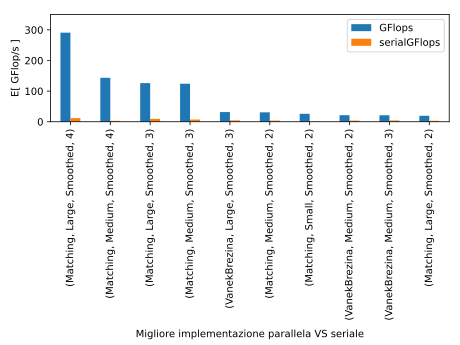
\includegraphics[width=.7\linewidth,keepaspectratio]{graphs/q4-b.svg.pdf}
\end{figure}

Variando il grado di parallelismo delle implementazioni parallele su alcuni input si è potuto
osservare come la migliore configurazione non è sempre quella con il numero di thread massimo, 
come è possibile notare dai grafici in figura \refbf{fig:q5},
ma è dipendente dalla dimensione della matrice e dal suo pattern di sparsità dei non zeri.
